\documentclass[10pt]{examdesign}
\usepackage{amsmath}
\usepackage{enumitem}
\usepackage{amsfonts}
\usepackage{pgfplots}
\usepackage{pifont}
\usepackage{graphicx}
\usepackage{fancyhdr}
\usepackage{cancel}
\usepackage{xcolor}
\SectionFont{\large\sffamily}
\Fullpages
\ContinuousNumbering


\DefineAnswerWrapper{}{}
\NumberOfVersions{1}
%\IncludeFromFile{foobar.tex}
\examname{Quiz A: Electrostatics}
\class{ {\Large AP Physics 2}}

\def \namedata {Name: \hrulefill\\ 
	Date: \hrulefill \\
	Period: \hrulefill \\
	Authentication Code: \hrulefill \\
	


	
}




\begin{document}




\begin{multiplechoice}
[title={Multiple Choice},
rearrange=no]
	\textit{Choose the best answer to each question.}
	\begin{question}
		The force exerted by a spring is given by $ F_s = -kx$.  What is the best explaination of the negative sign?
		\choice {The force of a spring is always in the negative direction.}
		\choice {A spring's force is always directed downward.}
		\choice [!]{The force of a spring is always opposite the direction it has been deformed.}
		\choice {A spring's force is always less than the force pulling on it.}
	\end{question}

	\begin{question}
	 	A spring is stretched a distance of 0.1 meters from its equilibrium position.  What kind of energy does the spring have?
		\choice [!] {Elastic Potential Energy}
		\choice {Gravitational Potential Energy}
		\choice {Kinetic Energy}
		\choice {Vernal Energy}
	\end{question}

	\begin{question}
		Which of the following could make a pendulum's period decrease?
		\choice {Decreasing the mass of the bob.}
		\choice {Increasing the maximum angle of the swing. }
		\choice [!]{Decreasing the length of the pendulum.}
		\choice {Decreasing the gravity acting on the pendulum.}
	\end{question}

	\begin{question}
		As a pendulum swings from one side of its path to the center, energy transforms - 
		\choice[!]{from gravitational potential energy to kinetic energy.}
		\choice{from gravitational potential energy to elastic potential energy.}
		\choice{from elastic potential energy to kinetic energy.}
		\choice{from kinetic energy to gravitational potential energy.}
	\end{question}


	\begin{question}
		A spring is stretched a distance of 3 cm and has an elastic potential energy of 2 J.  If the spring were to be stretched 9 cm, what would the elastic potential energy of the spring be? 
		\choice{2 J}
		\choice{6 J}
		\choice[!]{18 J}
		\choice{36 J}
	\end{question}
	
	\begin{question}
		Which of the following springs would be hardest to stretch or compress?
		\choice{A spring of spring constant $k = 10 \frac{N}{m}$}
		\choice{A spring of spring constant $k = 100 \frac{N}{m}$}
		\choice{A spring of spring constant $k = 1000 \frac{N}{m}$}
		\choice[!]{A spring of spring constant $k = 10000 \frac{N}{m}$}
	\end{question}
	
	\begin{question}
		Which is the best explanation of why old-fashioned clocks have pendulums?
		\choice[!]{The time it takes a pendulum to swing only depends on length and gravity.}
		\choice{The mass of a pendulum controls its period.}
		\choice{They can be used to hypnotize people while looking at the clock.}
		\choice{Pendulums look pretty.}
	\end{question}

	\begin{question}
		If the length of a pendulum is doubled, its period will - 
		\choice{remain the same}
		\choice[!]{increase by a factor of $\sqrt{2}$.}
		\choice{increase by a factor of 2.}
		\choice{Increase by a factor of 4.}
	\end{question}




	

	\end{multiplechoice}



\begin{shortanswer}[title={Free Response},
	rearrange=no]
	\begin{question}
	\vspace{-.2in}
		A student collects data from a spring, and finds the following: 
		 		 		 
		 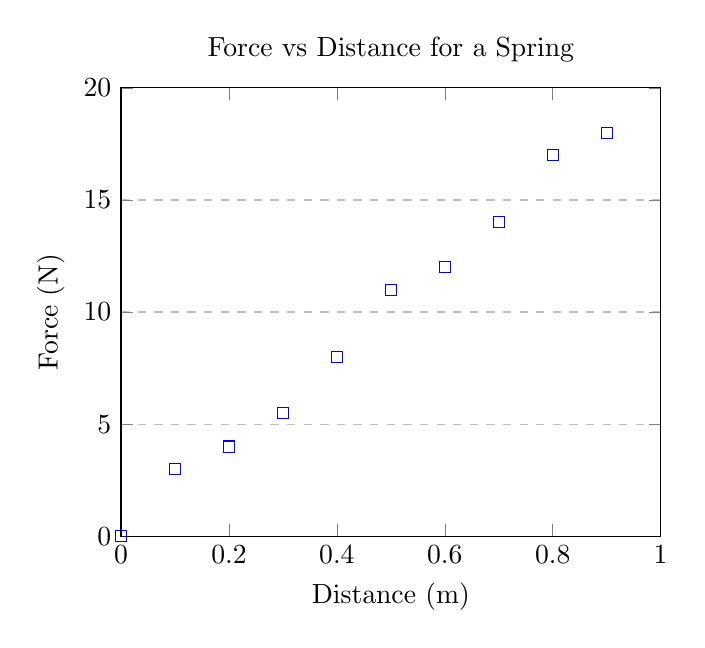
\begin{tikzpicture}
		 \begin{axis}[
		 title={Force vs Distance for a Spring},
		 xlabel={Distance (m)},
		 ylabel={Force (N)},
		 xmin=0, xmax=1,
		 ymin=0, ymax=20,
		 xtick={0,.20,.40,.60,.80,1},
		 ytick={0,5,10,15,20},
		 legend pos=north west,
		 ymajorgrids=true,
		 grid style=dashed,
		 ]
		 
		 \addplot[
		 color=blue,
		 only marks,
		 mark=square,
		 ]
		 coordinates {
		 	(0,0)(.1,3)(.2,4)(.3,5.5)(.4,8)(.5,11)(.6,12)(.7,14)(.8,17)(.9,18)
		 };
		 
		 \end{axis}
		 \end{tikzpicture}
		 
		 \begin{enumerate}
		 	\item Draw a best fit line through the data and find the slope of the line.
		 	\vspace{0.5in}	
		 	\item What is the Spring Constant of the Spring? 
		 	\vspace{.5in}
		 \end{enumerate}
		 
	
	\end{question}
	\begin{question}
	An astronaut wants to make a pendulum with a period of 1 second.  What would its length need to be on \word{{Mars}{Venus}} where gravity is \word{{3.8 $m/s^2$}{8.9 $m/s^2$}}?
	
		
	
	\end{question}
\end{shortanswer}

\end{document}
